\documentclass{article}
\usepackage[UTF8]{ctex}
\usepackage{amsmath,mathtools,geometry,pgfplots,float,mathrsfs,caption,enumerate}
\pgfplotsset{compat=1.15}
\usetikzlibrary{arrows}
\geometry{scale=0.7}

\title{每日一题(18.2)}
\author{\kaishu 程昊一}
\date{2022年5月25日}

\begin{document}
\maketitle
\begin{enumerate}
	\renewcommand{\labelenumi}{\textbf{\theenumi. }}
	\item 如图, 在四边形$ABCD$中, $AB\parallel CD$, $AC\perp BD$且$AC=BD$, $AC$与$BD$交于$O$. 过$O$做直线交$BC$于$M$, 交$AD$于$N$, $MN\perp BC$. 证明: $AD=2ON$. {\kaishu(原创题)}
	\begin{figure}[H]
		\flushright
		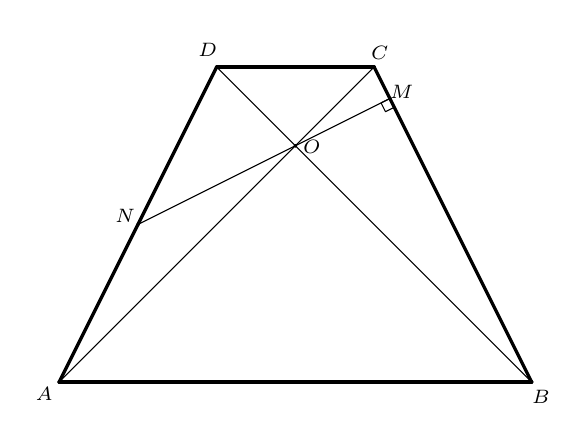
\begin{tikzpicture}[line cap=round,line join=round,>=triangle 45,x=1.0cm,y=1.0cm]
			\clip(-0.4,-0.4) rectangle (6.3,4.5);
			\draw[line width=0.4pt] (4.088414428162748,3.544207214081374) -- (4.144207214081374,3.4326216422441216) -- (4.255792785918627,3.4884144281627476) -- (4.2,3.6) -- cycle; 
			\draw [line width=1.2pt] (0.,0.)-- (6.,0.);
			\draw [line width=0.4pt] (0.,0.)-- (4.,4.);
			\draw [line width=0.4pt] (2.,4.)-- (6.,0.);
			\draw [line width=1.2pt] (6.,0.)-- (4.,4.);
			\draw [line width=1.2pt] (4.,4.)-- (2.,4.);
			\draw [line width=1.2pt] (2.,4.)-- (0.,0.);
			\draw [line width=0.4pt] (1.,2.)-- (4.2,3.6);
			\begin{scriptsize}
				\draw [fill=black] (0.,0.) circle (0.5pt);
				\draw[color=black] (-0.19101431316393505,-0.15180866768429746) node {$A$};
				\draw [fill=black] (6.,0.) circle (0.5pt);
				\draw[color=black] (6.119380253042317,-0.18709512378610318) node {$B$};
				\draw [fill=black] (3.,3.) circle (0.5pt);
				\draw[color=black] (3.208247624643347,2.988685925376412) node {$O$};
				\draw [fill=black] (4.,4.) circle (0.5pt);
				\draw[color=black] (4.072765799137587,4.182544356820839) node {$C$};
				\draw [fill=black] (2.,4.) circle (0.5pt);
				\draw[color=black] (1.8850055208256336,4.2119497369056775) node {$D$};
				\draw [fill=black] (1.,2.) circle (0.5pt);
				\draw[color=black] (0.8381739898053977,2.106524522831269) node {$N$};
				\draw [fill=black] (4.2,3.6) circle (0.5pt);
				\draw[color=black] (4.349176371935065,3.6826528953785913) node {$M$};
			\end{scriptsize}
		\end{tikzpicture}
	\end{figure}
	\item 如图, 在$\triangle ABC$中, $\angle BAC=60^\circ$. 平面上一点$O$, 满足$OA=OB=OC$. 过$O$作直线分别交$AB$, $AC$于$M$, $N$, 且满足$AM=AN$. 求证: $AB+AC=3MN$. {\kaishu(原创题)}
	\begin{figure}[H]
		\flushright
		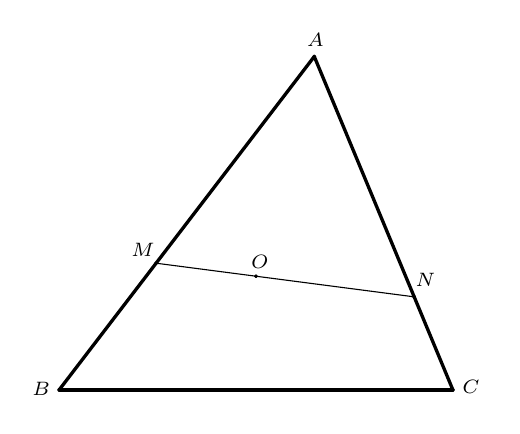
\begin{tikzpicture}[line cap=round,line join=round,>=triangle 45,x=1.0cm,y=1.0cm]
			\clip(-0.4,-0.2) rectangle (5.5,4.6);
			\draw [line width=1.2pt] (0.,0.)-- (3.2397854131350865,4.233725270398352);
			\draw [line width=1.2pt] (3.2397854131350865,4.233725270398352)-- (5.,0.);
			\draw [line width=1.2pt] (5.,0.)-- (0.,0.);
			\draw [line width=0.4pt] (1.231054827631172,1.6087324524201942)-- (4.508730585503915,1.1816171450040938);
			\begin{scriptsize}
				\draw [fill=black] (0.,0.) circle (0.5pt);
				\draw[color=black] (-0.2275066086937585,0.01800012524028992) node {$B$};
				\draw [fill=black] (5.,0.) circle (0.5pt);
				\draw[color=black] (5.231456584808791,0.03538535834061651) node {$C$};
				\draw [fill=black] (2.5,1.4433756729740645) circle (0.5pt);
				\draw[color=black] (2.5483356096583876,1.6232366481704452) node {$O$};
				\draw [fill=black] (3.2397854131350865,4.233725270398352) circle (0.5pt);
				\draw[color=black] (3.255335089071669,4.445439488123462) node {$A$};
				\draw [fill=black] (1.231054827631172,1.6087324524201942) circle (0.5pt);
				\draw[color=black] (1.0647957184305181,1.7739086683732759) node {$M$};
				\draw [fill=black] (4.508730585503915,1.1816171450040938) circle (0.5pt);
				\draw[color=black] (4.651948814797906,1.3914335401660907) node {$N$};
			\end{scriptsize}
		\end{tikzpicture}
	\end{figure}
\end{enumerate}
\end{document}